This chapter explore the method to further improve the performance levels of propsed load balancer.

The performance levels of L3DSR is discussed.
Then performance levels in the 10Gbps environment is discussed.
Novel XDP load balancer is discussed.


\section{L3DSR}

The ipvs has the mode called ipvs-tun, which is the so called Layer 3 Direct Server Return(l3dsr) functionality.
When the ipvs-tun send out the packets to real servers it encapsulates the original packet in ipip tunnling packet that is destined to real servers.
The realserver receives the packet on a tunl0 device and decapsulates the ipip packet, revealing the original packet.

\begin{figure}[h]
  \centering
  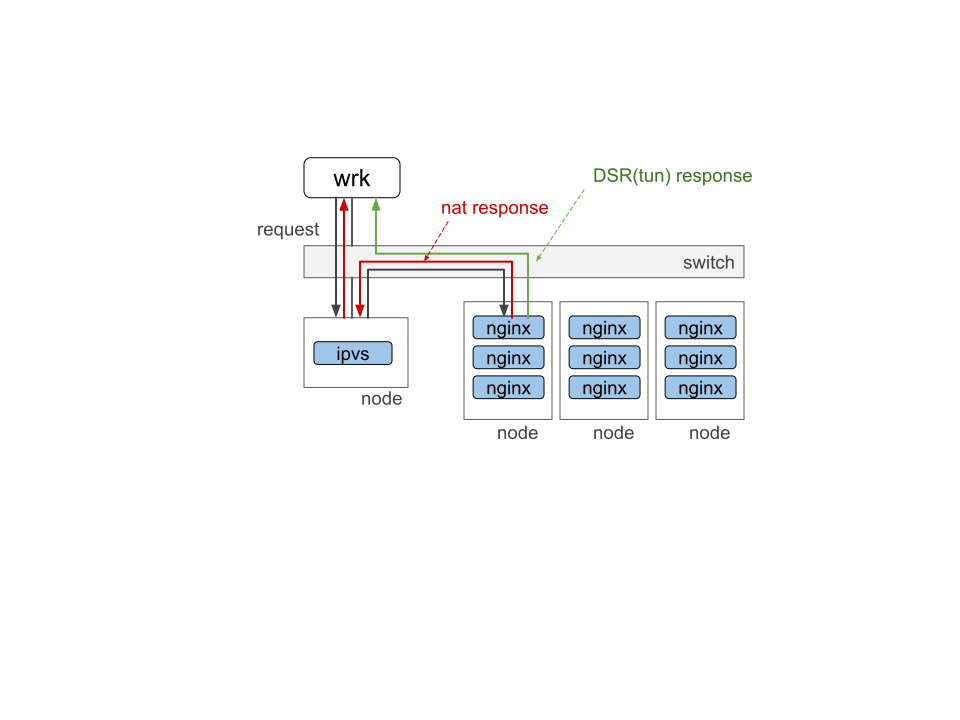
\includegraphics[width=0.8\columnwidth]{Figs/bench_1g_l3dsr}
  \caption{Physical configuration for L3DSR experiment.}
  \label{fig:bench_1g_l3dsr}
\end{figure}

\begin{figure}[h]
  \centering
  \includegraphics[width=0.8\columnwidth]{Figs/ipvs_l3dsr_1g.png}
  \caption{Throughput of ipvs l3dsr @1Gbps.}
  \label{fig:ipvs_l3dsr_1g.png}
\end{figure}

\FloatBarrier

\section{Load balancer for 10Gbps environment}

\begin{figure}[h]
  \centering
  \includegraphics[width=0.8\columnwidth]{Figs/bench_10g}
  \caption{Physical configuration for 10Gbps measurement.}
  \label{fig:bench_10g}
\end{figure}

\begin{figure}[h]
  \centering
  \includegraphics[width=0.8\columnwidth]{Figs/bench_10g_l3dsr}
  \caption{Physical configuration for L3DSR experiment.}
  \label{fig:bench_10g_l3dsr}
\end{figure}


\begin{figure}[t]
  \centering
  \includegraphics[width=0.8\columnwidth]{Figs/ipvs_l3dsr_10g.png}
  \caption{Throughput of ipvs l3dsr @10Gbps.}
  \label{fig:ipvs_l3dsr_10g.png}
\end{figure}

\FloatBarrier

\section{XDP load balancer}

\section{Summary}



